\documentclass{report}

\usepackage{graphicx}
\usepackage{algorithm}
\usepackage{array}
\usepackage{dsfont}
\usepackage{algpseudocode}
\usepackage{listings}
\usepackage{amsmath}
\usepackage{tikz}
\usepackage{pdfpages}
\usepackage{float}

\usetikzlibrary{automata, positioning, arrows}
\DeclareMathOperator{\rank}{rank}
\makeatletter
\newenvironment{sqcases}{%
  \matrix@check\sqcases\env@sqcases
}{%
  \endarray\right.%
}
\def\env@sqcases{%
  \let\@ifnextchar\new@ifnextchar
  \left\lbrack
  \def\arraystretch{1.2}%
  \array{@{}l@{\quad}l@{}}%
}
\makeatother

\usetikzlibrary{calc}


\input{/mnt/fa80f336-3342-4d78-8bfd-a43e434a2cda/Latex/preamble.tex}
\input{/mnt/fa80f336-3342-4d78-8bfd-a43e434a2cda/Latex/macros.tex}
\input{/mnt/fa80f336-3342-4d78-8bfd-a43e434a2cda/Latex/letterfonts.tex}

\title{\Huge{FU08 \-- Automata and Languages}\\Exercise 7}
\author{\huge{NGUYEN Tuan Dung}\\\huge{s1312004}}
\date{January 7, 2024}

\begin{document}

\maketitle

% Cau 1
\qs{Minimizing the following DFA}{
    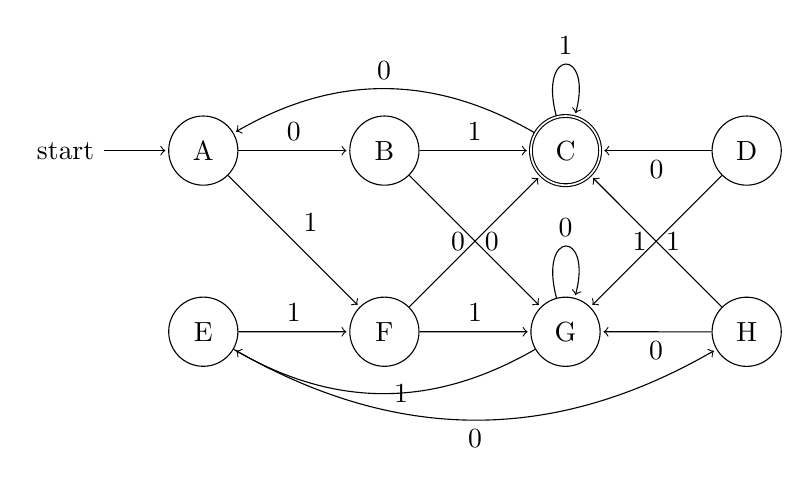
\begin{tikzpicture}[shorten >=1pt, scale=1.8, node distance=2.3cm, on grid, auto][h]
        \node[state, initial] (a) {A};
        \node[state] (b) [right=of a] {B};
        \node[state, accepting] (c) [right=of b] {C};
        \node[state] (d) [right=of c] {D};
        \node[state] (e) [below of=a] {E};
        \node[state] (f) [right=of e] {F};
        \node[state] (g) [right=of f] {G};
        \node[state] (h) [right=of g] {H};
    
        \path[->]   
        (a) edge node {0} (b)
            (a) edge node {1} (f)
        (b) edge node[right] {0} (g)
            (b) edge node {1} (c)
        (c) edge[bend right] node[above] {0} (a)
            (c) edge[loop above] node {1} (c)
        (d) edge node {0} (c)
            (d) edge node[left] {1} (g)
        (e) edge[bend right] node[below] {0} (h)
            (e) edge node {1} (f)
        (f) edge node[left] {0} (c)
            (f) edge node {1} (g)
        (g) edge[loop above] node {0} (g)
            (g) edge[bend left] node[above, right] {1} (e)
        (h) edge node {0} (g)
            (h) edge node[right] {1} (c);
    \end{tikzpicture}
}

\sol{\newline
Removing the useless state D. We reconstruct the DFA as.\\
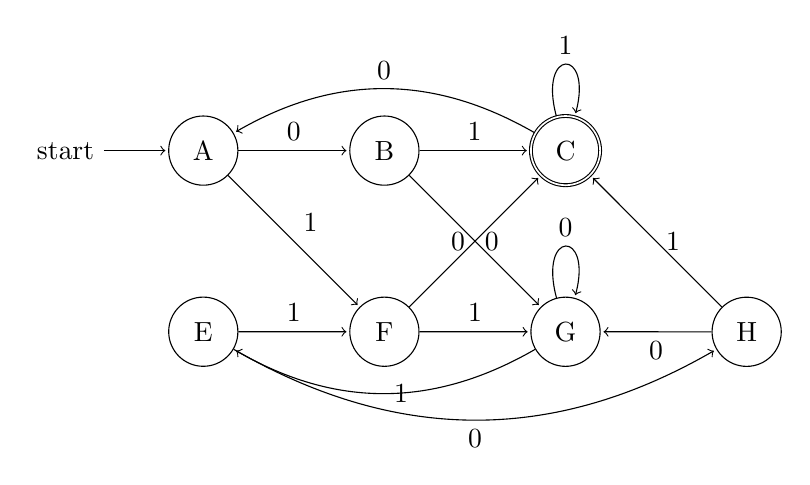
\begin{tikzpicture}[shorten >=1pt, scale=1.8, node distance=2.3cm, on grid, auto][h]
    \node[state, initial] (a) {A};
    \node[state] (b) [right=of a] {B};
    \node[state, accepting] (c) [right=of b] {C};
    \node[state] (e) [below of=a] {E};
    \node[state] (f) [right=of e] {F};
    \node[state] (g) [right=of f] {G};
    \node[state] (h) [right=of g] {H};

    \path[->]   
    (a) edge node {0} (b)
        (a) edge node {1} (f)
    (b) edge node[right] {0} (g)
        (b) edge node {1} (c)
    (c) edge[bend right] node[above] {0} (a)
        (c) edge[loop above] node {1} (c)
    (e) edge[bend right] node[below] {0} (h)
        (e) edge node {1} (f)
    (f) edge node[left] {0} (c)
        (f) edge node {1} (g)
    (g) edge[loop above] node {0} (g)
        (g) edge[bend left] node[above, right] {1} (e)
    (h) edge node {0} (g)
        (h) edge node[right] {1} (c);
\end{tikzpicture}
\newline
Using the DFA, we can construct a distinguishable table.
\begin{table}[h]
    \centering
    \begin{tabular}{|c|c|ccccc}
    \cline{1-2}
    B & F &                        &                        &                        &  &  \\ \cline{1-3}
    C & F & \multicolumn{1}{c|}{F} &                        &                        &  &  \\ \cline{1-4}
    E & T & \multicolumn{1}{c|}{F} & \multicolumn{1}{c|}{F} &                        &  &  \\ \cline{1-5}
    F & F & \multicolumn{1}{c|}{F} & \multicolumn{1}{c|}{F} & \multicolumn{1}{c|}{F} &  &  \\ \cline{1-6}
    G     & F & \multicolumn{1}{c|}{F} & \multicolumn{1}{c|}{F} & \multicolumn{1}{c|}{F} & \multicolumn{1}{c|}{F} &                        \\ \hline
    H     & F & \multicolumn{1}{c|}{T} & \multicolumn{1}{c|}{F} & \multicolumn{1}{c|}{F} & \multicolumn{1}{c|}{F} & \multicolumn{1}{c|}{F} \\ \hline
    state & A & \multicolumn{1}{c|}{B} & \multicolumn{1}{c|}{C} & \multicolumn{1}{c|}{E} & \multicolumn{1}{c|}{F} & \multicolumn{1}{c|}{G} \\ \hline
    \end{tabular}
    \caption{distinguishable table of the automaton}
\end{table}\newline
\textbf{Note}: T is True, F is False.\\
\begin{tikzpicture}[shorten >=1pt, scale=1.8, node distance=2.3cm, on grid, auto][h]
    \node[state, initial] (ae) {AE};
    \node[state] (bh) [right=of a] {BH};
    \node[state, accepting] (c) [right=of bh] {C};
    \node[state] (f) [below of=bh] {F};
    \node[state] (g) [below of=ae] {G};

    \path[->]   
    (ae) edge node {0} (bh)
        (ae) edge node[right] {1} (f)
    (bh) edge node[left] {0} (g)
        (bh) edge node {1} (c)
    (c) edge[loop above] node {1} (c)
        (c) edge[bend right] node[above] {1} (a)
    (g) edge[loop left] node {0} (g)
        (g) edge node {1} (ae)
    (f) edge node {0} (c)
        (f) edge node {1} (g);
\end{tikzpicture}
Note that $\delta(\mathrm{AE,1}) \mathrm{=F;~} \delta(\mathrm{BH,0}) \mathrm{=G}$. The automaton is minimal.
}
\pagebreak

% Cau 2
\qs{Minimize the following DFA}{
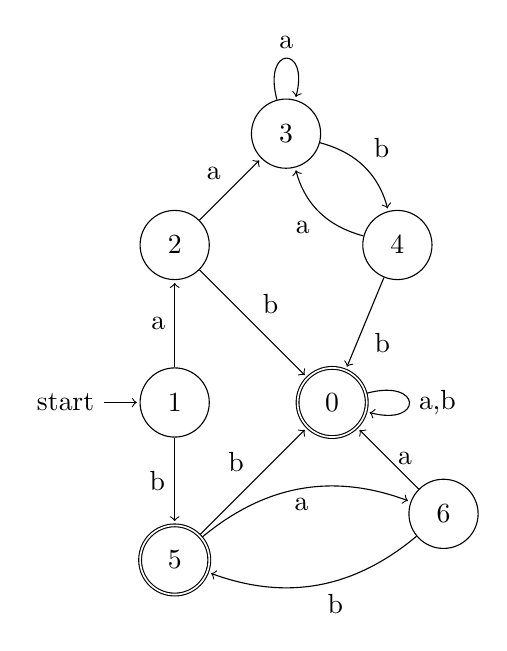
\begin{tikzpicture}[shorten >=1pt, node distance=2cm, on grid, auto][h]
    % Define states
    \node[state, initial] (q1)   {$1$};
    \node[state] (q2) [above=of q1] {$2$};
    \node[state] (q3) [above right=of q2] {$3$};
    \node[state] (q4) [below right=of q3] {$4$};
    \node[state, accepting] (q0) [right=of q1] {$0$};
    \node[state, accepting] (q5) [below=of q1] {$5$};
    \node[state] (q6) [below right=of q0] {$6$};
    
    % Define transitions
    \path[->]
    (q0) edge[loop right] node {a,b} (q0)
    (q1) edge node {a} (q2)
        (q1) edge node[left] {b} (q5)
    (q2) edge node {a} (q3)
        (q2) edge node {b} (q0)
    (q3) edge[loop above] node {a} (q3)
        (q3) edge[bend left] node {b} (q4)
    (q4) edge[bend left] node {a} (q3)
        (q4) edge node {b} (q0)
    (q5) edge[bend left] node[below] {a} (q6)
        (q5) edge node {b} (q0)
    (q6) edge node[right] {a} (q0)
        (q6) edge[bend left] node {b} (q5);
\end{tikzpicture}
}

\sol{\newline
Since there is no useless state in the DFA.\newline
\textbf{Immediately, we notice that}: 2 and 4 are equivalent.\\
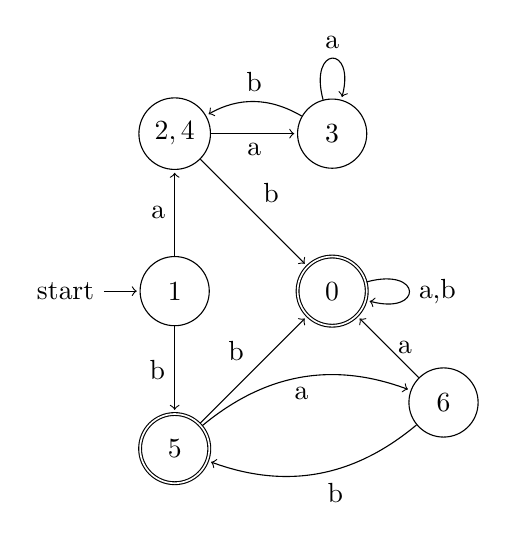
\begin{tikzpicture}[shorten >=1pt, node distance=2cm, on grid, auto][h]
    % Define states
    \node[state, initial] (q1)   {$1$};
    \node[state] (q24) [above=of q1] {$2,4$};
    \node[state] (q3) [right=of q24] {$3$};
    \node[state, accepting] (q0) [right=of q1] {$0$};
    \node[state, accepting] (q5) [below=of q1] {$5$};
    \node[state] (q6) [below right=of q0] {$6$};
    
    % Define transitions
    \path[->]
    (q0) edge[loop right] node {a,b} (q0)
    (q1) edge node {a} (q24)
        (q1) edge node[left] {b} (q5)
    (q24) edge node[below] {a} (q3)
        (q24) edge node {b} (q0)
    (q3) edge[loop above] node {a} (q3)
        (q3) edge[bend right] node[above] {b} (q24)
    (q5) edge[bend left] node[below] {a} (q6)
        (q5) edge node {b} (q0)
    (q6) edge node[right] {a} (q0)
        (q6) edge[bend left] node {b} (q5);
\end{tikzpicture}
\newline
Since there are no obvious sign of equivalency, we construct a distinguishable table.\\
\textbf{Note}: T is True, F is False.\newline
\begin{table}[h]
    \centering
    \begin{tabular}{|c|c|cccc}
    \cline{1-2}
    1   & F &                        &                        &  &  \\ \cline{1-3}
    2,4 & F & \multicolumn{1}{c|}{F} &                        &  &  \\ \cline{1-4}
    3   & F & \multicolumn{1}{c|}{F} & \multicolumn{1}{c|}{F} &  &  \\ \cline{1-5}
    5     & F & \multicolumn{1}{c|}{F} & \multicolumn{1}{c|}{F}   & \multicolumn{1}{c|}{F} &                        \\ \hline
    6     & F & \multicolumn{1}{c|}{F} & \multicolumn{1}{c|}{F}   & \multicolumn{1}{c|}{F} & \multicolumn{1}{c|}{F} \\ \hline
    state & 0 & \multicolumn{1}{c|}{1} & \multicolumn{1}{c|}{2,4} & \multicolumn{1}{c|}{3} & \multicolumn{1}{c|}{5} \\ \hline
    \end{tabular}
    \caption{distinguishable table of the automaton}
    \end{table}
\newline
From this table, we agree that the automaton is indeed minimal.
}
\pagebreak

% Cau 3
\qs{Minimize the DFA}{
$M=\left(Q, \sum, \delta, q_0, F\right) \text { with }\\
Q=\left\{q_0, q_1, q_2, q_3, q_4, q_5, q_6, q_7\right\} \\
\sum=\{0,1\} \\
F=\left\{q_3\right\}, \text { and } \delta \text { is defined by }$
\newline
$$
\begin{array}{|l|l|l|}
\hline \delta & 0 & 1 \\
\hline \mathrm{q}_0 & \mathrm{q}_1 & \mathrm{q}_0 \\
\hline \mathrm{q}_1 & \mathrm{q}_0 & \mathrm{q}_2 \\
\hline \mathrm{q}_2 & \mathrm{q}_3 & \mathrm{q}_1 \\
\hline \mathrm{q}_3 & \mathrm{q}_3 & \mathrm{q}_0 \\
\hline \mathrm{q}_4 & \mathrm{q}_3 & \mathrm{q}_5 \\
\hline \mathrm{q}_5 & \mathrm{q}_6 & \mathrm{q}_4 \\
\hline \mathrm{q}_6 & \mathrm{q}_5 & \mathrm{q}_6 \\
\hline \mathrm{q}_7 & \mathrm{q}_6 & \mathrm{q}_3 \\
\hline
\end{array}
$$
}

\sol{\newline
From the above transition table, we construct a DFA out of it.\newline
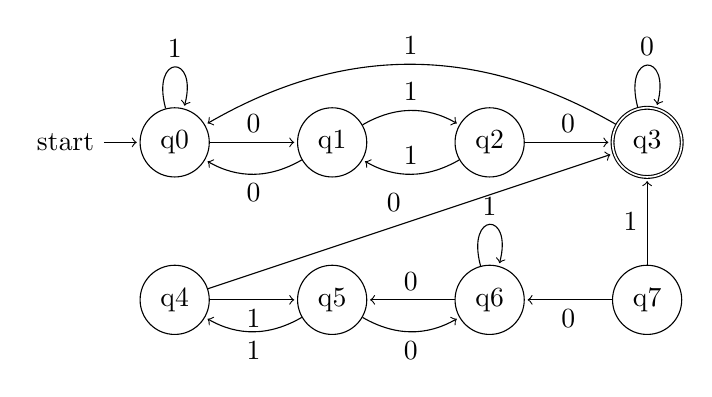
\begin{tikzpicture}[shorten >=1pt, node distance=2cm, on grid, auto][h]
    % Define states
    \node[state, initial] (q0)   {q0};
    \node[state] (q1) [right=of q0] {q1};
    \node[state] (q2) [right=of q1] {q2};
    \node[state, accepting] (q3) [right=of q2] {q3};
    \node[state] (q4) [below of=q0] {q4};
    \node[state] (q5) [right=of q4] {q5};
    \node[state] (q6) [right=of q5] {q6};
    \node[state] (q7) [right=of q6] {q7};
    
    % Define transitions
    \path[->]
    (q0) edge node[above] {0} (q1)
        (q0) edge[loop above] node {1} (q0)
    (q1) edge[bend left] node {0} (q0)
        (q1) edge[bend left] node {1} (q2)
    (q2) edge node[above] {0} (q3)
        (q2) edge[bend left] node[above] {1} (q1)
    (q3) edge[loop above] node {0} (q3)
        (q3) edge[bend right] node[above] {1} (q0)
    (q4) edge node {0} (q3)
        (q4) edge node[below] {1} (q5)
    (q5) edge[bend right] node[below] {0} (q6)
        (q5) edge[bend left] node {1} (q4)
    (q6) edge node[above] {0} (q5)
        (q6) edge[loop above] node {1} (q6)
    (q7) edge node {0} (q6)
        (q7) edge node {1} (q3);
\end{tikzpicture}
\newline
Immediately, we notice the useless state q4,q5,q6,q7. Removing the useless states. We reconstruct the DFA as.\\
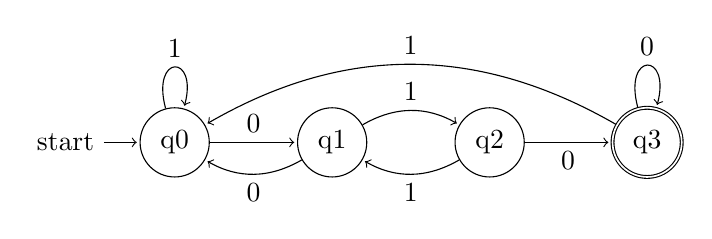
\begin{tikzpicture}[shorten >=1pt, node distance=2cm, on grid, auto][h]
    % Define states
    \node[state, initial] (q0)   {q0};
    \node[state] (q1) [right=of q0] {q1};
    \node[state] (q2) [right=of q1] {q2};
    \node[state, accepting] (q3) [right=of q2] {q3};
    
    % Define transitions
    \path[->]
    (q0) edge node[above] {0} (q1)
        (q0) edge[loop above] node {1} (q0)
    (q1) edge[bend left] node {0} (q0)
        (q1) edge[bend left] node {1} (q2)
    (q2) edge node[below] {0} (q3)
        (q2) edge[bend left] node[below] {1} (q1)
    (q3) edge[loop above] node {0} (q3)
        (q3) edge[bend right] node[above] {1} (q0);
\end{tikzpicture}
\newline
From the DFA, we construct a distinguishable table for the automaton.\\
\begin{table}[h]
    \centering
    \begin{tabular}{|c|c|cc}
    \cline{1-2}
    1     & F &                        &                        \\ \cline{1-3}
    2     & F & \multicolumn{1}{c|}{F} &                        \\ \hline
    3     & F & \multicolumn{1}{c|}{F} & \multicolumn{1}{c|}{F} \\ \hline
    state & 0 & \multicolumn{1}{c|}{1} & \multicolumn{1}{c|}{2} \\ \hline
    \end{tabular}
    \caption{distinguishable table of the automaton}
    \end{table}
\newline
\noindent We conclude that the automaton is minimal.
}
\end{document}
